% Options for packages loaded elsewhere
\PassOptionsToPackage{unicode}{hyperref}
\PassOptionsToPackage{hyphens}{url}
%
\documentclass[
]{article}
\usepackage{lmodern}
\usepackage{amssymb,amsmath}
\usepackage{ifxetex,ifluatex}
\ifnum 0\ifxetex 1\fi\ifluatex 1\fi=0 % if pdftex
  \usepackage[T1]{fontenc}
  \usepackage[utf8]{inputenc}
  \usepackage{textcomp} % provide euro and other symbols
\else % if luatex or xetex
  \usepackage{unicode-math}
  \defaultfontfeatures{Scale=MatchLowercase}
  \defaultfontfeatures[\rmfamily]{Ligatures=TeX,Scale=1}
\fi
% Use upquote if available, for straight quotes in verbatim environments
\IfFileExists{upquote.sty}{\usepackage{upquote}}{}
\IfFileExists{microtype.sty}{% use microtype if available
  \usepackage[]{microtype}
  \UseMicrotypeSet[protrusion]{basicmath} % disable protrusion for tt fonts
}{}
\makeatletter
\@ifundefined{KOMAClassName}{% if non-KOMA class
  \IfFileExists{parskip.sty}{%
    \usepackage{parskip}
  }{% else
    \setlength{\parindent}{0pt}
    \setlength{\parskip}{6pt plus 2pt minus 1pt}}
}{% if KOMA class
  \KOMAoptions{parskip=half}}
\makeatother
\usepackage{xcolor}
\IfFileExists{xurl.sty}{\usepackage{xurl}}{} % add URL line breaks if available
\IfFileExists{bookmark.sty}{\usepackage{bookmark}}{\usepackage{hyperref}}
\hypersetup{
  pdftitle={Introduction to R and RMarkdown},
  hidelinks,
  pdfcreator={LaTeX via pandoc}}
\urlstyle{same} % disable monospaced font for URLs
\usepackage[margin=1in]{geometry}
\usepackage{color}
\usepackage{fancyvrb}
\newcommand{\VerbBar}{|}
\newcommand{\VERB}{\Verb[commandchars=\\\{\}]}
\DefineVerbatimEnvironment{Highlighting}{Verbatim}{commandchars=\\\{\}}
% Add ',fontsize=\small' for more characters per line
\usepackage{framed}
\definecolor{shadecolor}{RGB}{248,248,248}
\newenvironment{Shaded}{\begin{snugshade}}{\end{snugshade}}
\newcommand{\AlertTok}[1]{\textcolor[rgb]{0.94,0.16,0.16}{#1}}
\newcommand{\AnnotationTok}[1]{\textcolor[rgb]{0.56,0.35,0.01}{\textbf{\textit{#1}}}}
\newcommand{\AttributeTok}[1]{\textcolor[rgb]{0.77,0.63,0.00}{#1}}
\newcommand{\BaseNTok}[1]{\textcolor[rgb]{0.00,0.00,0.81}{#1}}
\newcommand{\BuiltInTok}[1]{#1}
\newcommand{\CharTok}[1]{\textcolor[rgb]{0.31,0.60,0.02}{#1}}
\newcommand{\CommentTok}[1]{\textcolor[rgb]{0.56,0.35,0.01}{\textit{#1}}}
\newcommand{\CommentVarTok}[1]{\textcolor[rgb]{0.56,0.35,0.01}{\textbf{\textit{#1}}}}
\newcommand{\ConstantTok}[1]{\textcolor[rgb]{0.00,0.00,0.00}{#1}}
\newcommand{\ControlFlowTok}[1]{\textcolor[rgb]{0.13,0.29,0.53}{\textbf{#1}}}
\newcommand{\DataTypeTok}[1]{\textcolor[rgb]{0.13,0.29,0.53}{#1}}
\newcommand{\DecValTok}[1]{\textcolor[rgb]{0.00,0.00,0.81}{#1}}
\newcommand{\DocumentationTok}[1]{\textcolor[rgb]{0.56,0.35,0.01}{\textbf{\textit{#1}}}}
\newcommand{\ErrorTok}[1]{\textcolor[rgb]{0.64,0.00,0.00}{\textbf{#1}}}
\newcommand{\ExtensionTok}[1]{#1}
\newcommand{\FloatTok}[1]{\textcolor[rgb]{0.00,0.00,0.81}{#1}}
\newcommand{\FunctionTok}[1]{\textcolor[rgb]{0.00,0.00,0.00}{#1}}
\newcommand{\ImportTok}[1]{#1}
\newcommand{\InformationTok}[1]{\textcolor[rgb]{0.56,0.35,0.01}{\textbf{\textit{#1}}}}
\newcommand{\KeywordTok}[1]{\textcolor[rgb]{0.13,0.29,0.53}{\textbf{#1}}}
\newcommand{\NormalTok}[1]{#1}
\newcommand{\OperatorTok}[1]{\textcolor[rgb]{0.81,0.36,0.00}{\textbf{#1}}}
\newcommand{\OtherTok}[1]{\textcolor[rgb]{0.56,0.35,0.01}{#1}}
\newcommand{\PreprocessorTok}[1]{\textcolor[rgb]{0.56,0.35,0.01}{\textit{#1}}}
\newcommand{\RegionMarkerTok}[1]{#1}
\newcommand{\SpecialCharTok}[1]{\textcolor[rgb]{0.00,0.00,0.00}{#1}}
\newcommand{\SpecialStringTok}[1]{\textcolor[rgb]{0.31,0.60,0.02}{#1}}
\newcommand{\StringTok}[1]{\textcolor[rgb]{0.31,0.60,0.02}{#1}}
\newcommand{\VariableTok}[1]{\textcolor[rgb]{0.00,0.00,0.00}{#1}}
\newcommand{\VerbatimStringTok}[1]{\textcolor[rgb]{0.31,0.60,0.02}{#1}}
\newcommand{\WarningTok}[1]{\textcolor[rgb]{0.56,0.35,0.01}{\textbf{\textit{#1}}}}
\usepackage{graphicx,grffile}
\makeatletter
\def\maxwidth{\ifdim\Gin@nat@width>\linewidth\linewidth\else\Gin@nat@width\fi}
\def\maxheight{\ifdim\Gin@nat@height>\textheight\textheight\else\Gin@nat@height\fi}
\makeatother
% Scale images if necessary, so that they will not overflow the page
% margins by default, and it is still possible to overwrite the defaults
% using explicit options in \includegraphics[width, height, ...]{}
\setkeys{Gin}{width=\maxwidth,height=\maxheight,keepaspectratio}
% Set default figure placement to htbp
\makeatletter
\def\fps@figure{htbp}
\makeatother
\usepackage[normalem]{ulem}
% Avoid problems with \sout in headers with hyperref
\pdfstringdefDisableCommands{\renewcommand{\sout}{}}
\setlength{\emergencystretch}{3em} % prevent overfull lines
\providecommand{\tightlist}{%
  \setlength{\itemsep}{0pt}\setlength{\parskip}{0pt}}
\setcounter{secnumdepth}{-\maxdimen} % remove section numbering

\title{Introduction to R and RMarkdown}
\author{}
\date{\vspace{-2.5em}2020-01-06}

\begin{document}
\maketitle

{
\setcounter{tocdepth}{2}
\tableofcontents
}
\hypertarget{rmarkdown}{%
\section{RMarkdown}\label{rmarkdown}}

RMarkdown is a combination of two tools: Markdown is a simple way of
writing plain text that can be formatted into fancy documents. Markdown
originated as a tool for easily writing blog posts and comments that
include formatting, such as section headings, italic and bold-faced
text, and so forth without having to learn a technical formatting
language, such as HTML. Markdown is fairly generic, so it is easy to
translate a single Markdown document into many output formats, such as
HTML for web pages, PDF, and Microsoft Word documents.

You can learn a lot about the details of Markdown at the RStudio web
site \url{http://rmarkdown.rstudio.com}. RStudio has a handy cheat sheet
for RMarkdown that you can see by opening the Help menu, going to
``Cheatsheets'' and opening the RMarkdown Cheat Sheet or the more
comprehensive RMarkdown Reference.

What makes RMarkdown different from ordinary Markdown is that it allows
you to combine text, formatted in Markdown, with instructions to the R
statistical software to analyze data and produce graphs, tables, and
other useful output.

By integrating the data analysis with the text of a document, we can
easily make our research reproducible. The RMarkdown file contains all
the instructions to load the data, analyze it, and generate the final
report. Then if your data changes and you need to update your report,
you can do so by knitting the RMarkdown document with the updated data
files.

To turn an RMarkdown document into an HTML, PDF, or Microsoft Word
document, you just click on the ``Knit'' button in RStudio. If you click
on the word ``Knit'' on the button, RStudio will turn the RMarkdown
document into the default format (see below). To knit the document into
a different output format, click on the arrow just to the right of the
word ``Knit,'' and select the output format you want.

I use RMarkdown to produce all of the documents I produce for the labs
in this course. You can see my code at
\url{https://github.com/gilligan-ees-3310-2018}. The code for all of the
Lab \#1 documentation is at
\url{https://github.com/gilligan-ees-3310-2018/lab_01_documentation}

\hypertarget{document-header}{%
\section{Document header}\label{document-header}}

At the top of an RMarkdown document there is a section set off by lines
of three hyphens above it and below it.

Here is an example:

\begin{verbatim}
---
title: "Your document's title"
subtitle: "Your document's subtitle"
author: "Your name goes here"
date: "Aug 28, 2017"
output:
    pdf_document: default
    html_document: default
---
\end{verbatim}

By default, when RStudio knits the document, it converts it into the
format listed first under \texttt{output\_format}

When the output format lists, for instance,
``\texttt{pdf\_format:\ default}'', that means that when RStudio creates
a pdf document, it uses the default options. If you want to customize
the output, you can specify options for RStudio to use in creating PDF,
HTML, or Word output documents:

\begin{verbatim}
---
title: "Your document's title"
subtitle: "Your document's subtitle"
author: "Your name goes here"
date: "Aug 28, 2017"
output:
    pdf_document:
      toc: "true" 
      number_sections: "false"
    html_document:
      self_contained: "false"
---
\end{verbatim}

\hypertarget{markdown}{%
\section{Markdown}\label{markdown}}

Some of the basic elements of Markdown are:

\hypertarget{paragraphs}{%
\subsection{Paragraphs}\label{paragraphs}}

Any block of one or more lines of text, with a blank line before and a
blank line after is treated as a single paragraph. To separate
paragraphs, put a blank line between them:

\hypertarget{markdown-1}{%
\subsubsection{Markdown:}\label{markdown-1}}

\begin{verbatim}
This is one paragraph.
It stretches over several consecutive lines,
but it will be formatted 
as a single paragraph.

This is another paragraph.
The blank line between the two
blocks of text tells Markdown
that they are separate paragraphs
\end{verbatim}

\hypertarget{formatted-output}{%
\subsubsection{Formatted Output:}\label{formatted-output}}

\begin{quote}
This is one paragraph. It stretches over several consecutive lines, but
it will be formatted as a single paragraph.

This is another paragraph. The blank line between the two blocks of text
tells Markdown that they are separate paragraphs
\end{quote}

\hypertarget{section-headers}{%
\subsection{Section headers}\label{section-headers}}

Any line of text that begins with one or more hash symbols (``\#'') and
is preceded by a blank line is treated as a section header. Top-level
section headers have a single hash, and subsections, subsubsections,
etc. use two, three, etc. hashes.

\hypertarget{markdown-2}{%
\subsubsection{Markdown:}\label{markdown-2}}

\begin{verbatim}
# This is a top-level section header

## This is a subsection

### This is a subsubsection

# This is another section
\end{verbatim}

\hypertarget{formatted-output-1}{%
\subsubsection{Formatted Output:}\label{formatted-output-1}}

\begin{verbatim}
\end{verbatim}

\begin{quote}
\hypertarget{this-is-a-top-level-section-header}{%
\section{This is a top-level section
header}\label{this-is-a-top-level-section-header}}

\hypertarget{this-is-a-subsection}{%
\subsection{This is a subsection}\label{this-is-a-subsection}}

\hypertarget{this-is-a-subsubsection}{%
\subsubsection{This is a subsubsection}\label{this-is-a-subsubsection}}

\hypertarget{this-is-another-section}{%
\section{This is another section}\label{this-is-another-section}}
\end{quote}

\hypertarget{formatting-text}{%
\subsection{Formatting text}\label{formatting-text}}

To make \emph{italic text} and \textbf{boldface text} you surround the
text with underscores or asterisks. A single underscore or asterisk
means italic, two means boldface, and three means both italic and
boldface:

\hypertarget{markdown-3}{%
\subsubsection{Markdown:}\label{markdown-3}}

\begin{verbatim}
This is _italic text_. This is *also italic text*. __This is boldface__ and 
**so is this**. ***This is bold italic***. This is ~~strikethrough~~, perhaps 
to indicate an error.
\end{verbatim}

\hypertarget{formatted-output-2}{%
\subsubsection{Formatted Output:}\label{formatted-output-2}}

\begin{quote}
This is \emph{italic text}. This is \emph{also italic text}.
\textbf{This is boldface} and \textbf{so is this}. \textbf{\emph{This is
bold italic}}. This is \sout{strikethrough}, perhaps to indicate an
error.
\end{quote}

\hypertarget{lists}{%
\subsection{Lists}\label{lists}}

You can make bulleted or numbered lists easily in Markdown. Simply begin
a line with an asterisk, hyphen, or plus sign. To make a sub-list, just
indent the lines of the sublist by four spaces.

\hypertarget{markdown-4}{%
\subsubsection{Markdown:}\label{markdown-4}}

\begin{verbatim}
* This is a list

* This is the second item of the list.

    * This is a sub-list

    * This is another item in the sub-list
    
        A list item can have several paragraphs. Just ident the continuation 
        by four additional spaces and do not begin it with an asterisk.
        If you have multiple lines with no blank line separating them,
        Markdown treats them as a single paragraph.

        Here is a third paragraph of continuation.

* This is the main list again.
  Just as with other things, you can break a single list item into several lines,
  and as long as there is no blank line between them, Markdown knows to treat
  them as a single paragraph.
\end{verbatim}

\hypertarget{formatted-output-3}{%
\subsubsection{Formatted Output:}\label{formatted-output-3}}

\begin{itemize}
\item
  This is a list
\item
  This is the second item of the list.

  \begin{itemize}
  \item
    This is a sub-list
  \item
    This is another item in the sub-list

    A list item can have several paragraphs. Just indent the
    continuation by four additional spaces and do not begin it with an
    asterisk. If you have multiple lines with no blank line separating
    them, Markdown treats them as a single paragraph.

    Here is a third paragraph of continuation.
  \end{itemize}
\item
  This is the main list again. Just as with other things, you can break
  a single list item into several lines, and as long as there is no
  blank line between them, Markdown knows to treat them as a single
  paragraph.
\end{itemize}

\hypertarget{numbered-lists}{%
\subsection{Numbered Lists}\label{numbered-lists}}

To make numbered lists, start them with a number and a period:

\hypertarget{markdown-5}{%
\subsubsection{Markdown}\label{markdown-5}}

\begin{verbatim}
1. This is a list

1. This is the second item of the list. Notice that I keep using the 
   numeral "1", but Markdown automatically increments the numbers
   for the list items.

    a) This is a sub-list

    a) This is another item in the sub-list
    
        A list item can have several paragraphs.
        
        Here is a third paragraph of continuation.
        
        i) this is a sub-sub list numbered with Roman numerals

        i) this is a sub-sub list numbered with Roman numerals

        i) this is a sub-sub list numbered with Roman numerals

1. This is the main list again.
\end{verbatim}

\hypertarget{formatted-output-4}{%
\subsubsection{Formatted Output:}\label{formatted-output-4}}

\begin{enumerate}
\def\labelenumi{\arabic{enumi}.}
\item
  This is a list
\item
  This is the second item of the list. Notice that I keep using the
  numeral ``1'', but Markdown automatically increments the numbers for
  the list items.

  \begin{enumerate}
  \def\labelenumii{\alph{enumii})}
  \item
    This is a sub-list
  \item
    This is another item in the sub-list

    A list item can have several paragraphs.

    Here is a third paragraph of continuation.

    \begin{enumerate}
    \def\labelenumiii{\roman{enumiii})}
    \item
      this is a sub-sub list numbered with Roman numerals
    \item
      this is a sub-sub list numbered with Roman numerals
    \item
      this is a sub-sub list numbered with Roman numerals
    \end{enumerate}
  \end{enumerate}
\item
  This is the main list again.
\end{enumerate}

\hypertarget{mathematical-expressions}{%
\subsection{Mathematical expressions}\label{mathematical-expressions}}

For simple math, you can just type stuff in RMarkdown:
\texttt{1\ +\ 2\ *\ 3} comes out as 1 + 2 * 3. If you want subscripts or
superscripts, you can get those by using the \texttt{\textasciitilde{}}
and \texttt{\^{}} characters, respectively:
\texttt{I\textasciitilde{}out\textasciitilde{}\ =\ sigma\ T\^{}4\^{}}
appears as I\textsubscript{out} = sigma T\textsuperscript{4}.

If you want fancier formatting for mathematical expressions, RMarkdown
has a way to do this.

If you put an expression between dollar signs, RMarkdown interprets it
differently from regular RMarkdown, and uses a format called LaTeX that
is used for typesetting sophisticated mathematics. I won't try to
present all of LaTeX here, but will give some common examples:

An expression between single dollar signs is interpreted as
\emph{in-line} math that appears in the middle of a line of text. LaTeX
uses special terms that begin with a backslash \texttt{\textbackslash{}}
to indicate special mathematical formatting or operators. For example
\texttt{\$a\ +\ b\ \textbackslash{}times\ x\$} appears as
\(a + b \times x\).

You can show Greek letters, like \(\alpha\), \(\pi\), and \(\sigma\) by
spelling them out like this: \texttt{\$\textbackslash{}alpha\$},
\texttt{\$\textbackslash{}pi\$}, and \texttt{\$\textbackslash{}sigma\$}.
The epsilon that we use to indicate emissivity is a variation on the
ordinary Greek epsilon, so we spell it
\texttt{\$\textbackslash{}varepsilon\$} to get \(\varepsilon\).

LaTeX handles subscripts and superscripts differently from RMarkdown:
You use \texttt{\_\{\}} and \texttt{\^{}\{\}} with whatever you want to
appear in the subscript or superscript inside the braces \texttt{\{\}}:
\texttt{\$I\_\{out\}\ =\ \textbackslash{}sigma\ T\^{}\{4\}\$} appears as
\(I_{out} = \sigma T^{4}\)

You can include square root signs using \texttt{\textbackslash{}sqrt}:
\texttt{\$x\ =\ \textbackslash{}sqrt\{y\ \textbackslash{}times\ z\}\$}
appears as \(x = \sqrt{y \times z}\). You can do other roots like this:
\texttt{\$T\ =\ \textbackslash{}sqrt{[}4{]}\{I\_\{out\}\ /\ \textbackslash{}sigma\}\$}
appears as \(T = \sqrt[4]{I_{out} / \sigma}\).

To get display math, which appears on its own line, you use double
dollar signs. This is useful when you want to write a mathematical
expression that is much taller than a line of text. In display mode you
can display fractions using
\texttt{\textbackslash{}frac\{numerator\ expression\}\{denominator\ expression\}},
as in this example:
\texttt{\$\$\textbackslash{}varepsilon\ \textbackslash{}sigma\ T\^{}4\ =\ \textbackslash{}frac\{(1\ -\ \textbackslash{}alpha)\}\{4\}\ \textbackslash{}times\ I\_\{solar\}\$\$}
appears as

\[ \varepsilon \sigma T^4 = \frac{(1 - \alpha)}{4} \times I_{solar}\]
\texttt{\$\$T\_\{bare\ rock\}\ =\ \textbackslash{}sqrt{[}4{]}\{\textbackslash{}frac\{(1\ -\ \textbackslash{}alpha)\}\{4\ \textbackslash{}varepsilon\ \textbackslash{}sigma\}\ \textbackslash{}times\ I\_\{solar\}\}\$\$}
appears as

\[T_{bare rock} = \sqrt[4]{\frac{(1 - \alpha)}{4 \varepsilon \sigma} \times I_{solar}}\]

There is a lot more to the LaTeX notation that you can use in RMarkdown,
but what I have shown here is sufficient for everything you will do in
this class. You won't need to use this kind of mathematical notation
very much, but it can be convenient, especially when you are working
exercises on atmospheric layer models.

If you find it too difficult to use LaTeX mathematical notation, I will
accept either hand-written supplements in which you write out the
equations by hand, or a textual description in your document where you
use words instead of mathematical symbols to explain what you are doing.

\hypertarget{figures}{%
\subsection{Figures}\label{figures}}

You can include image files in your RMarkdown document:

\hypertarget{markdown-6}{%
\subsubsection{Markdown}\label{markdown-6}}

\begin{verbatim}
![This is a tornado](images/tornado.jpg)
\end{verbatim}

\hypertarget{formatted-output-5}{%
\subsubsection{Formatted Output:}\label{formatted-output-5}}

\begin{figure}
\centering

\includegraphics{images/tornado.jpg}
\caption{This is a tornado}
\end{figure}

\hypertarget{hyperlinks}{%
\subsection{Hyperlinks}\label{hyperlinks}}

You can include links to documents on the web in two ways. The simplest
is if you want the URL for the link to appear in your document you can
just surround the URL with angle brackets:
\texttt{\textless{}https://www.vanderbilt.edu\textgreater{}} appears as
\url{https://www.vanderbilt.edu}.

If you want to add a hyperlink to some text in your document, then you
would do it like this:

\begin{verbatim}
[Vanderbilt University](https://www.vanderbilt.edu)
\end{verbatim}

to get this: \href{https://www.vanderbilt.edu}{Vanderbilt University}.

Note the difference between the hyperlink specification and the image
specification is whether there is an exclamation point before the square
brackets.

\hypertarget{using-r-for-calculations}{%
\section{Using R for calculations}\label{using-r-for-calculations}}

RMarkdown combines the ``Markdown'' system for formatting text with the
R statistical system for performing calculations and making graphs.

We are using R for the laboratory section of this course because it
allows you to easily analyze large amounts of data and produce
high-quality graphs.

To enter R expressions in an RMarkdown document, we use ``code blocks''
and ``inline code''. Code blocks are useful if we are doing a
calculation, and inline code is useful if you just want to insert a
number (maybe one you have calculated in a code block) into the middle
of a line of text.

Code blocks begin and end with three consecutive ``back-tick''
characters:

Inline code appears between single back-ticks:
\texttt{\textasciigrave{}r\ code\ goes\ here\textasciigrave{}}

We express basic mathematical operations in R similarly to the way we
express them in Excel and most programming languages. Addition and
subtraction use the normal plus and minus signs. Multiplication uses an
asterisk, division uses a slash (``/''), and powers (exponentiation)
uses ``\^{}''.

R has a lot of mathematical functions you can use, such as
\texttt{sqrt()}, \texttt{log()} (for the natural logarithm),
\texttt{log10()} for the base-10 logarithm, and so forth.

We can assign numbers to variables using the equals sign:

\begin{Shaded}
\begin{Highlighting}[]
\NormalTok{sigma =}\StringTok{ }\FloatTok{5.67E-8}
\NormalTok{I_solar =}\StringTok{ }\DecValTok{1350} \CommentTok{# watts per square meter}
\NormalTok{albedo =}\StringTok{ }\FloatTok{0.3}
\NormalTok{I_absorbed =}\StringTok{ }\NormalTok{I_solar }\OperatorTok{*}\StringTok{ }\NormalTok{(}\DecValTok{1} \OperatorTok{-}\StringTok{ }\NormalTok{albedo)}
\NormalTok{T =}\StringTok{ }\NormalTok{(I_absorbed }\OperatorTok{/}\StringTok{ }\NormalTok{(}\DecValTok{4} \OperatorTok{*}\StringTok{ }\NormalTok{sigma))}\OperatorTok{^}\FloatTok{0.25}
\end{Highlighting}
\end{Shaded}

If the last line of a code block is something with a value (e.g., the
name of a variable or a mathematical expression, as opposed to an
assignment with an equals sign), then R will show that value:

\begin{Shaded}
\begin{Highlighting}[]
\NormalTok{T}
\end{Highlighting}
\end{Shaded}

\begin{verbatim}
## [1] 254.0664
\end{verbatim}

We can also print the value of an R expression in the middle of a line
of text using inline code: \texttt{T\ =}
\texttt{\textasciigrave{}r\ T\textasciigrave{}} will give T =
254.0663741.

Inline code is very useful because it lets us ask R to automatically
insert a number into the text. This means that every time we knit the
document, that number is generated by R. If you write a report and then
realize that there was a problem with the data or the analysis, you can
just fix the problem and re-knit the report using the corrected data and
analysis code. You don't need to manually go through a separate document
and edit the numbers to update them with the latest results from your
analysis. RMarkdown will do that for you, if you used inline code to
insert the numbers into your text.

Thus, a bit of extra work at the beginning to set up the document and
analysis using RMarkdown saves lots of time later on by making it
trivial to update the document.

Code blocks also allow us to include graphs in our document:

\begin{figure}
\centering
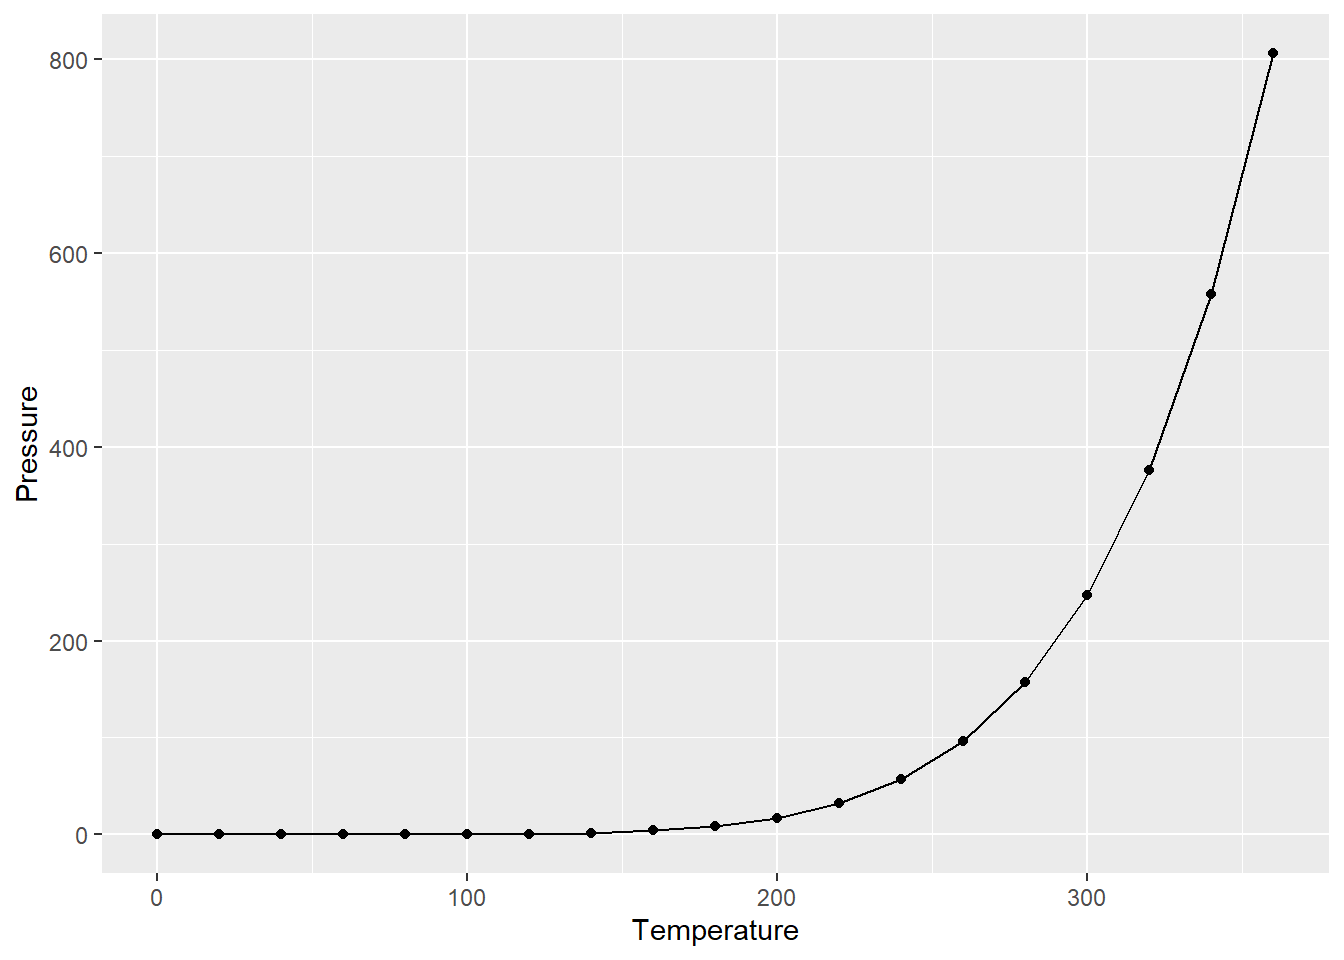
\includegraphics{lab_01_rmarkdown_intro_files/figure-latex/graph_example-1.pdf}
\caption{This is a plot of pressure versus temperature.}
\end{figure}

\hypertarget{loading-r-scripts}{%
\subsection{Loading R Scripts}\label{loading-r-scripts}}

In this course, I am trying to teach you to use the basics of R.
Sometimes we will need to do things for our analysis that require more
complicated R programming, and then I will write R scripts that contain
this code so you don't need to write it yourself from scratch, but can
just call functions that I provide.

To load a script (a file containing R code), you use the R command
\texttt{source("script\_file.R"")}

For the exercises here, we will use two scripts, which are located in
the "\_scripts" directory.

To load them into R so you can use them in your analysis, you would put
the following code into your RMarkdown document:

\begin{Shaded}
\begin{Highlighting}[]
\KeywordTok{source}\NormalTok{(}\StringTok{"_scripts/format_md.R"}\NormalTok{)}
\KeywordTok{source}\NormalTok{(}\StringTok{"_scripts/layer_diagram.R"}\NormalTok{)}
\end{Highlighting}
\end{Shaded}

\hypertarget{useful-scripts-for-the-labs}{%
\subsubsection{Useful Scripts for the
Labs:}\label{useful-scripts-for-the-labs}}

These first script defines a function, \texttt{format\_md}, which
formats numbers nicely for markdown documents, allowing you to control
how many significant digits it shows, and optionally using scientific
notation or inserting commas to separate thousands, millions, etc.

\texttt{format\_md(sigma,\ digits\ =\ 1)} will produce 0.00000006

\texttt{format\_md(pi\ *\ 1E6,\ digits\ =\ 3,\ format="scientific")}
will produce 3.142×10\textsuperscript{6}

\texttt{format\_md(pi\ *\ 1E6,\ digits\ =\ 3,\ comma\ =\ TRUE)} will
produce 3,142,000

\hypertarget{script-for-layer-diagrams}{%
\subsubsection{Script for Layer
Diagrams}\label{script-for-layer-diagrams}}

The other script allows you to produce a layer diagram, similar to the
ones in Chapter 3 of \emph{Global Warming: Understanding the Forecast}.

\begin{Shaded}
\begin{Highlighting}[]
\KeywordTok{make_layer_diagram}\NormalTok{(}\DecValTok{2}\NormalTok{)}
\end{Highlighting}
\end{Shaded}

\begin{verbatim}
## Warning: `data_frame()` is deprecated, use `tibble()`.
## This warning is displayed once per session.
\end{verbatim}

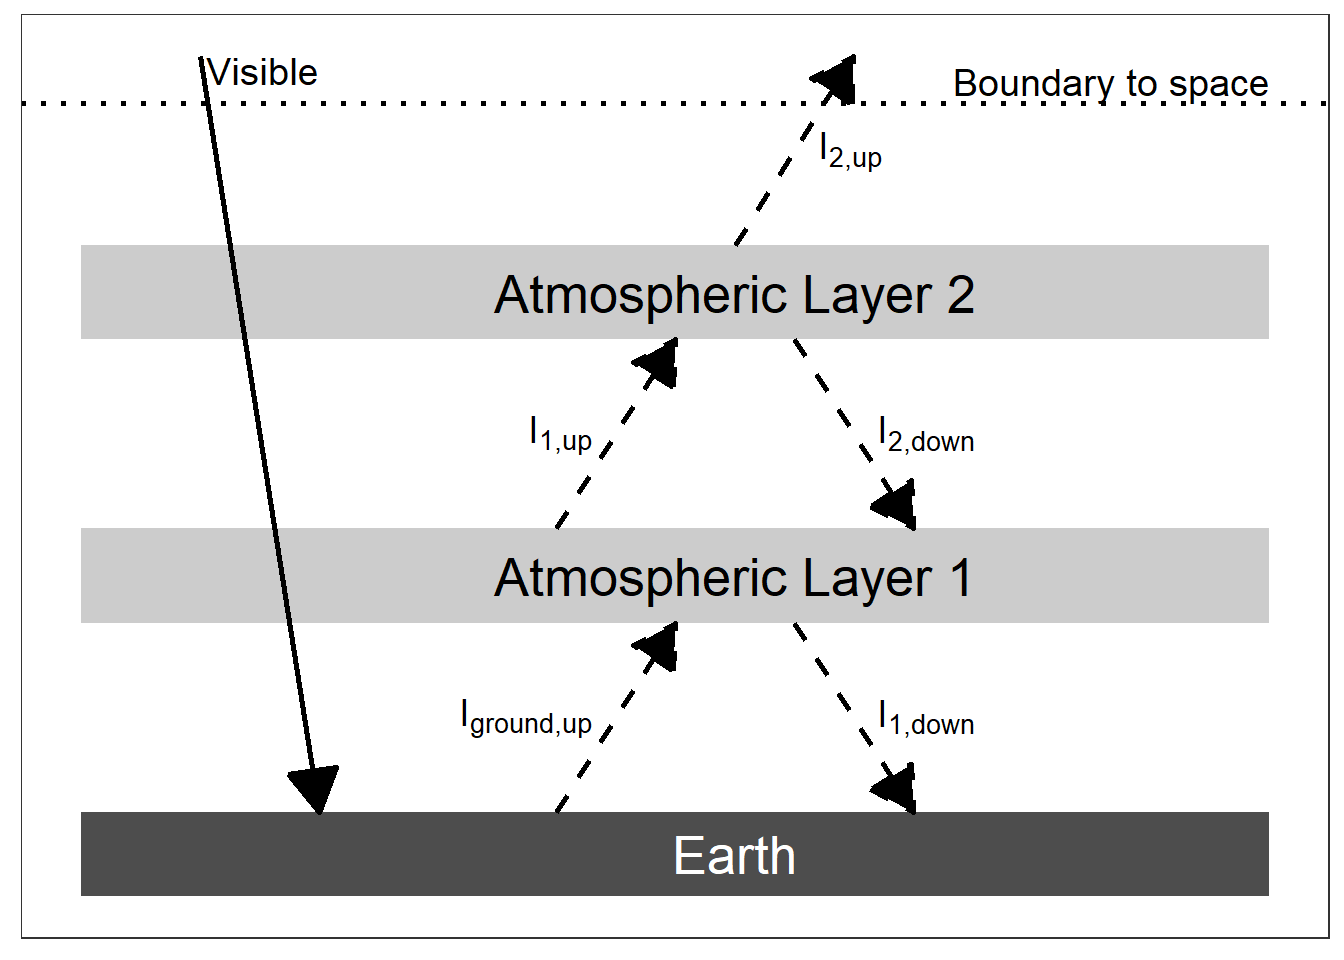
\includegraphics{lab_01_rmarkdown_intro_files/figure-latex/example_layer_diagram-1.pdf}

\end{document}
